\section*{Trigonometry}

\subsection*{Unit Circle}
\begin{Figure}
	\centering
	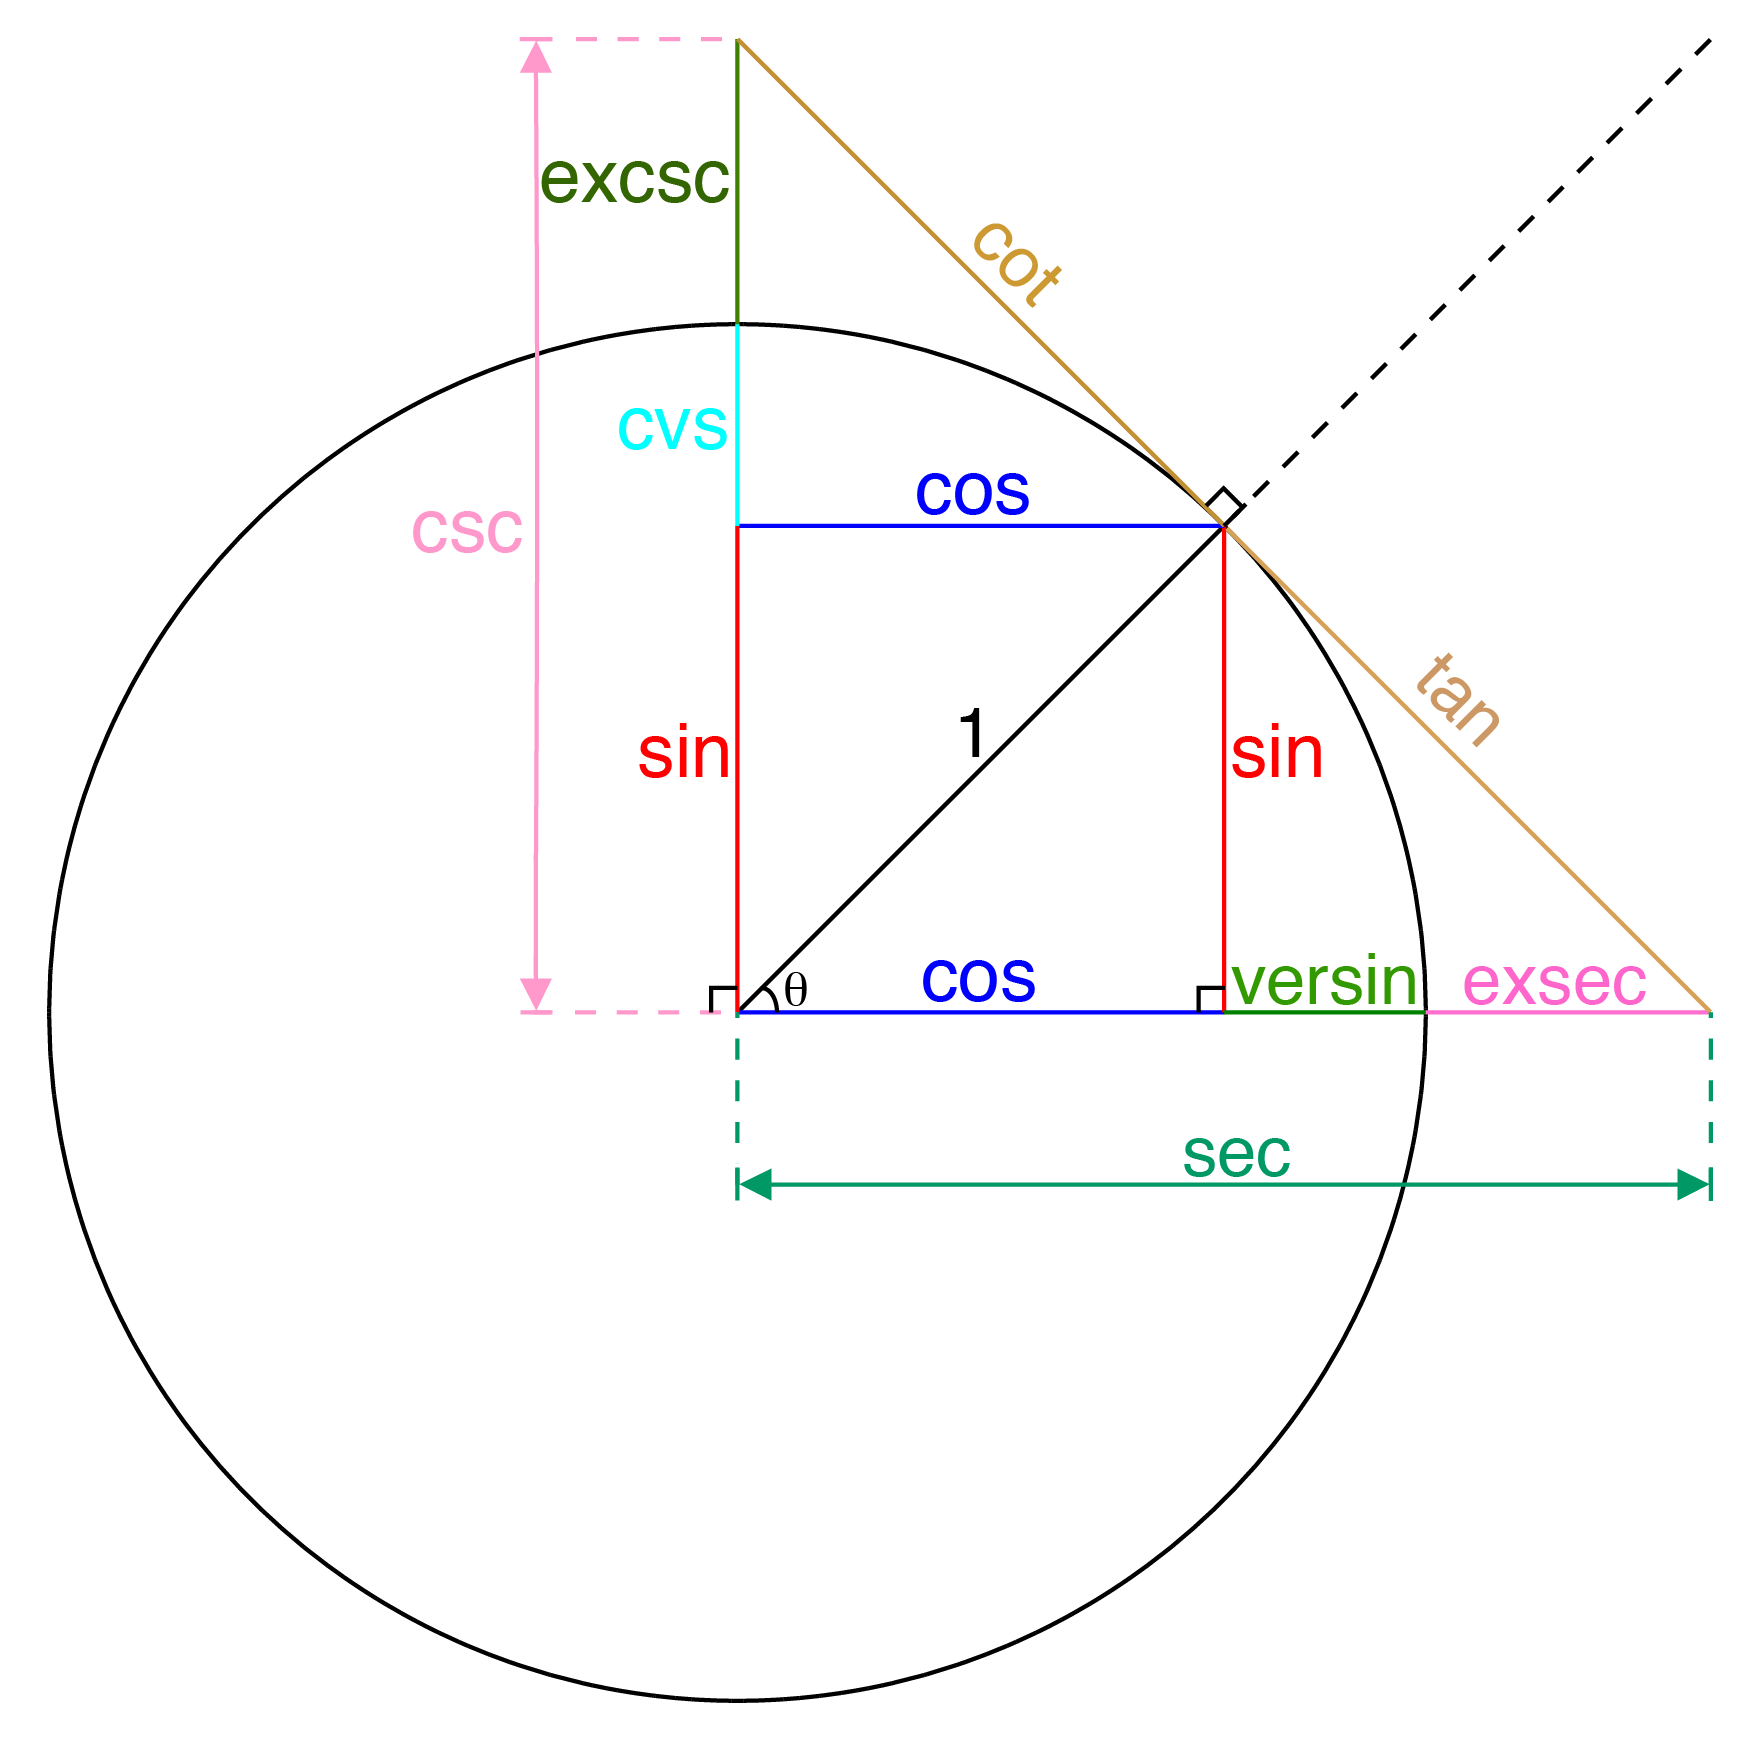
\includegraphics[width=\linewidth]{circle}
	%\captionof{figure}{my caption of the figure}
\end{Figure}
\subsection*{Domain and Range}
\begin{itemize}[leftmargin=0.5em, label={�}]
	\item $\sin:\R\longrightarrow[-1,1]$
	\item $\cos:\R\longrightarrow[-1,1]$
	\item $\tan = \frac{\sin}{\cos}:\left\{x \in \R \ \middle| \ x \neq \frac{\pi}{2} + k\pi\right\}\longrightarrow\R$
	\item $\cot = \frac{1}{\tan} : \left\{x \in \R \ \middle| \ x \neq k\pi\right\}\longrightarrow\R$
	\item $\csc = \frac{1}{\sin} :\left\{x \in \R \ \middle| \ x \neq k\pi\right\}\longrightarrow\R \setminus \left(-1,1\right)$
	\item $\sec = \frac{1}{\cos} :\left\{x \in \R \ \middle| \ x \neq \frac{\pi}{2} + k\pi\right\}\longrightarrow\R \setminus \left(-1,1\right)$
	\item $\sin^{-1}: \left[-1,1\right] \longrightarrow \left[-\frac{\pi}{2},\frac{\pi}{2}\right]$
	\item $\cos^{-1}: \left[-1,1\right] \longrightarrow \left[0,\pi\right]$		
	\item $\tan^{-1}: \R \longrightarrow \left[-\frac{\pi}{2},\frac{\pi}{2}\right]$
\end{itemize}
\subsection*{Pythagorean Identities}	
\begin{eqlist}
	\item $\sin^2(x) + \cos^2(x) = 1$
	\item $\tan^2(x) + 1 = \sec^2(x)$
	\item $1 + \cot^2(x) = \csc^2(x)$
\end{eqlist}


\subsection*{Quotient Identities}	
\begin{eqlist}
	\item $\tan(x) = \frac{\sin(x)}{\cos(x)}$
	\item $\cot(x) = \frac{\cos(x)}{\sin(x)}$
\end{eqlist}

\subsection*{Sum Identities}	
\begin{eqlist}
	\item $\sin(x + y) = \sin(x)\cos(y) + \cos(x)\sin(y)$
	\item $\cos(x + y) = \cos(x)\cos(y) - \sin(x)\sin(y)$
	\item $\tan(x + y) = \frac{\tan(x) + \tan(y)}{1-\tan(x)\tan(y)}$
\end{eqlist}

\subsection*{Difference Identities}	
\begin{eqlist}
	\item $\sin(x - y) = \sin(x)\cos(y) - \cos(x)\sin(y)$
	\item $\cos(x - y) = \cos(x)\cos(y) + \sin(x)\sin(y)$
	\item $\tan(x - y) = \frac{\tan(x) - \tan(y)}{1 + \tan(x)\tan(y)}$
\end{eqlist}

\subsection*{Double Angle Identities}	
\begin{eqlist}
	\item $\sin(2x) = 2\sin(x)\cos(x)$
	\item $\cos(2x) = \cos^2(x) - \sin^2(x) $
	\item $\cos(2x) = 2\cos^2(x) - 1 \Rightarrow \cos^2(x) = \frac{\cos(2x)+1}{2}$
	\item $\cos(2x) = 1 - 2\sin^2(x) \Rightarrow \sin^2(x) = \frac{1-\cos(2x)}{2}$
	\item $\tan(2x) = \frac{2\tan(x)}{1-\tan^2(x)} $
\end{eqlist}

\subsection*{Co-Function Identities}	
\begin{eqlist}
	\item $\sin\left(\frac{\pi}{2}-x\right) = \cos(x)$
	\item $\cos\left(\frac{\pi}{2}-x\right) = \sin(x)$
	\item $\tan\left(\frac{\pi}{2}-x\right) = \cot(x)$
	\item $\cot\left(\frac{\pi}{2}-x\right) = \tan(x)$
	\item $\csc\left(\frac{\pi}{2}-x\right) = \sec(x)$	
	\item $\sec\left(\frac{\pi}{2}-x\right) = \csc(x)$
\end{eqlist}

\subsection*{Even-Odd Identities}	
\begin{eqlist}
	\item $\sin(-x) = -\sin(x)$
	\item $\cos(-x) = \cos(x)$
	\item $\tan(-x) = -\tan(x)$
	\item $\cot(-x) = -\cot(x)$
	\item $\csc(-x) = -\csc(x)$
	\item $\sec(-x) = \sec(x)$
\end{eqlist}

\subsection*{Half-Angle Identities}	
\begin{eqlist}
	\item $\sin\left(\frac{x}{2}\right) = \pm\sqrt{\frac{1-\cos(x)}{2}}$
	\item $\cos\left(\frac{x}{2}\right) = \pm\sqrt{\frac{1+\cos(x)}{2}}$
	\item $\tan\left(\frac{x}{2}\right) = \pm\sqrt{\frac{1-\cos(x)}{2}}$
	\item $\tan\left(\frac{x}{2}\right) = \frac{1-\cos(x)}{\sin(x)}$
	\item $\tan\left(\frac{x}{2}\right) = \frac{\sin(x)}{1+\cos(x)}$
\end{eqlist}

\subsection*{Sum-to-Product Formulas}
\begin{eqlist}
	\item $\sin(x) + \sin(y) = 2\sin\left(\frac{x+y}{2}\right)\cos\left(\frac{x-y}{2}\right)$
	\item $\sin(x) - \sin(y) = 2\sin\left(\frac{x-y}{2}\right)\cos\left(\frac{x+y}{2}\right)$
	\item $\cos(x) + \cos(y) = 2\cos\left(\frac{x+y}{2}\right)\cos\left(\frac{x-y}{2}\right)$
	\item $\cos(x) - \cos(y) = -2\sin\left(\frac{x+y}{2}\right)\cos\left(\frac{x-y}{2}\right)$
\end{eqlist}

\subsection*{Product-to-Sum Formulas}
\begin{eqlist}
	\item $\sin(x)\sin(y) = \frac{1}{2}\left[\cos(x-y)-\cos(x+y)\right]$
	\item $\cos(x)\cos(y) = \frac{1}{2}\left[\cos(x-y)+\cos(x+y)\right]$
	\item $\sin(x)\cos(y) = \frac{1}{2}\left[\sin(x+y)+\sin(x-y)\right]$
	\item $\cos(x)\sin(y) = \frac{1}{2}\left[\sin(x+y)-\sin(x-y)\right]$
\end{eqlist}


\subsection*{Laws of Sines}
\begin{eqlist}
	\item $\frac{\sin(\alpha)}{a} = \frac{\sin(\beta)}{b} = \frac{\sin(\gamma)}{c}$
\end{eqlist}

\subsection*{Laws of Cosines}
\begin{eqlist}
	\item $a^2 = b^2 + c^2 - 2bc\cos(\alpha)$
	\item $b^2 = a^2 + c^2 - 2ac\cos(\beta)$
	\item $c^2 = a^2 + b^2 - 2ab\cos(\gamma)$
\end{eqlist}

\subsection*{Degrees}
\begin{Figure}
	\centering
	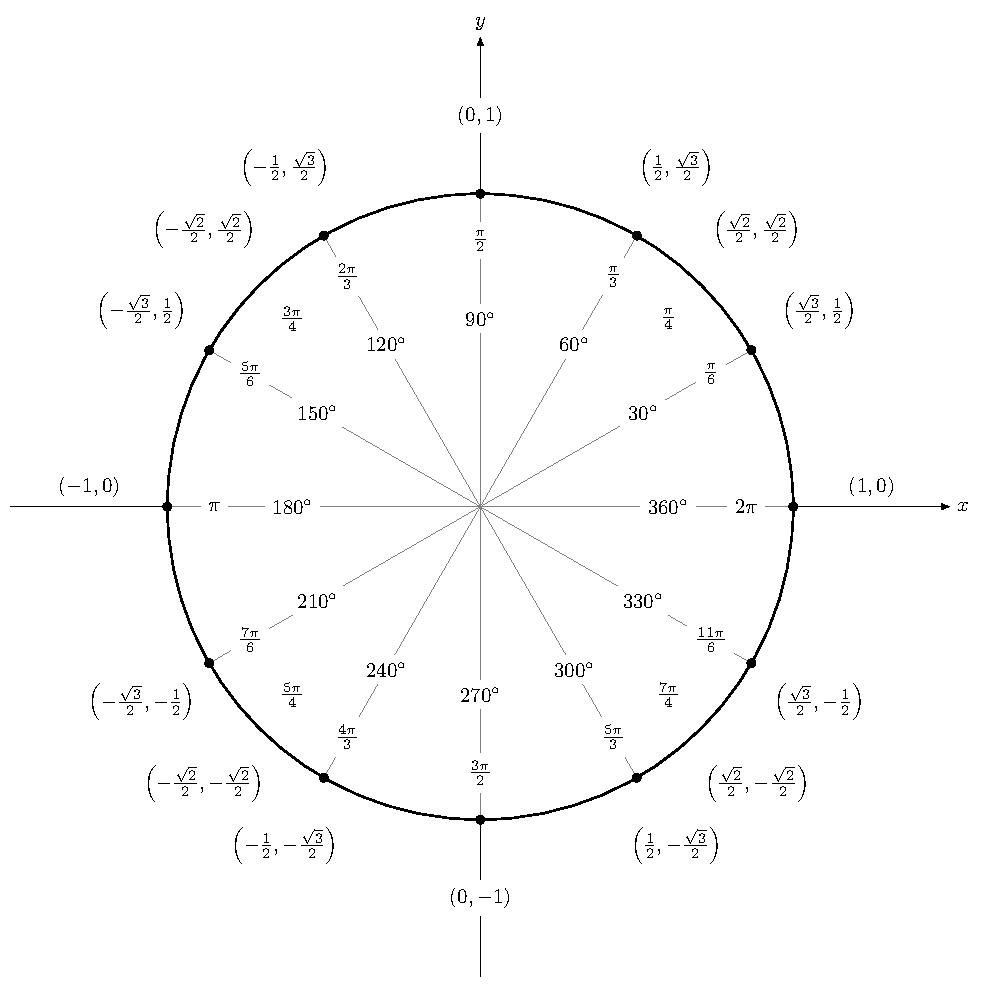
\includegraphics[width=\linewidth]{degrees_circle}
	%\captionof{figure}{my caption of the figure}
\end{Figure}

\begin{Figure}
	\centering
	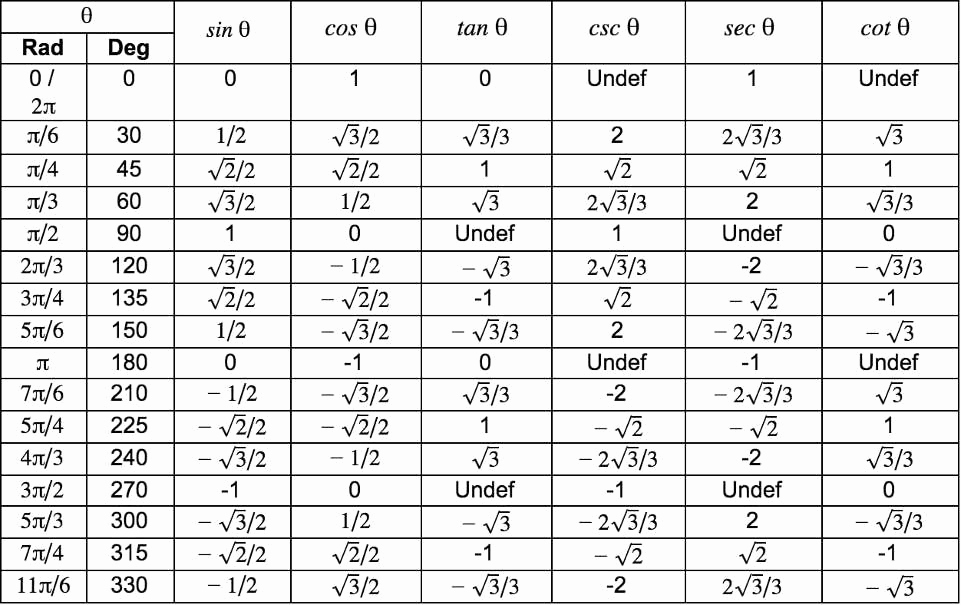
\includegraphics[width=\linewidth]{unit_circle_table}
\end{Figure}
